\documentclass[a4paper,oneside,12pt]{article}
\usepackage[utf8]{inputenc}
\usepackage{dcolumn}
\usepackage[spanish]{babel}

\usepackage{graphicx}

\begin{document}

\pagenumbering{arabic}

\title{CRefactory}
\author{Baglivo Nicol\'as C\'esar \and Costa Federico Daniel \and Perera Nicanor Gonzalo \and Szeinfeld Matias Ezequiel \and Tarragona Juan Pablo}
\date{\today}
\maketitle

\tableofcontents

\newpage

\section{Organizaci\'on del documento}
Primero se dar\'a una introducci\'on para poner en contexto al problema planteado por la c\'atedra junto con la  motivaci\'on para la realizaci\'on del trabajo. Se detallar\'an los objetivos del mismo as\'i como tambi\'en la manera de trabajo del grupo.

Luego, se ir\'an detallando en orden de aparici\'on los problemas con los que nos fuimos enfrentando a lo largo de la cursada. Por cada uno de ellos se explicar\'a en que consiste junto a la soluci\'on planteada.

Mas adelante se listar\'a un resumen de las minutas de cada reuni\'on con la Profesora.
Por \'ultimo se detallar\'an las conclusiones y el trabajo a futuro.

\section{Introducci\'on}
La refactorizaci\'on de c\'odigo es una t\'ecnica para la reestructuraci\'on del c\'odigo existente de un producto de software, alterando su estructura interna sin cambiar su comportamiento externo, con el objetivo de mejorar atributos no funcionales del software como pueden ser la legibilidad, la mantenibilidad o incluso la extensibidad del mismo.

Existe una serie de t\'ecnicas bien conocidas de uso com\'un durante el proceso de refactorizaci\'on de c\'odigo, CRefactory es un entorno de desarrollo que provee soporte para realizar de manera autom\'atica los aspectos mec\'anicos de dicho proceso mediante una interfaz gr\'afica.

Crefactory esta programado en Smalltalk dentro del entorno de desarrollo VisualWorks. La interfaz gr\'afica que posee la aplicaci\'on permite interactuar con c\'odigo C para facilitar dicha refactorizaci\'on. 

Permite refactorizar variables (cambio de nombre, crear estructuras de las variables), estructuras (renombrar campos) y funciones (renombrar las mismas).

\subsection{Motivaci\'on}
CRefactory funcionaba correctamente, pero estaba lejos de ser la herramienta ideal de trabajo, ya que su interfaz no era amigable con el usuario. En primer lugar, la carga de archivos era muy poco pr\'actica, ya que era necesario escribir el path de los archivos a mano, y no se pose\'ia ning\'un tipo de retroalimentaci\'on para saber si se hab\'ia referenciado correctamente dicho archivo. Se vi\'o la necesidad de mejorar la manera en que se cargaraban los archivos.

En segundo lugar, la herramienta no era capaz de agregar condiciones falsas o macros por medio de la interfaz, con lo cual se desaprovechaba  parte del poder de CRefactory. Era necesario implementar esto de una manera amigable al usuario por medio de una interfaz gr\'afica.

En tercer lugar, no se entend\'ia que ocurr\'ia en caso de que se produjera una excepci\'on. Se necesitaba implementar una manera f\'acil y amigable para que se traten las mismas y as\'i detectar el error. Se necesitaba un mejor manejo de las excepciones y una interfaz para tratarlas.

Por ejemplo, si ocurr\'ia un error durante el parseo de un archivo, no mostraba el contenido del mismo y por ende no mostraba la l\'inea de c\'odigo que produjo el error. Por lo que tambi\'en fue necesario implementar resaltado de sint\'axis para la detecci\'on de error en parseo.


\subsection{Objetivos}

Mejorar la experiencia del usuario al utilizar la herramienta haciendo \'enfasis en su facilidad de uso, proveer retroalimentaci\'on, manejo de excepciones, di\'alogo simple y natural, salidas evidentes, prevenci\'on de errores y ayudas.

Particularmente se desea mejorar la carga de archivos e include\_directories para que cumpla las siguientes condiciones: prevenci\'on de errores, facilidad de uso, simplicidad y menor sorpresa al usuario.

Implementar una interfaz que permita al usuario el manejo de macros y condiciones falsas de una manera sencilla e intuitiva, de manera que pueda agregarlas o quitarlas a gusto.

Desarrollar una manera de visualizar la ocurrencia de errores y excepciones que sea adecuada, clara y funcional. Debe permitir reconocer r\'apidamente al agente que causa el error y que provea suficiente informaci\'on para que el usuario pueda resolverlo.

\subsection{Manera de trabajo}

Para realizar el trabajo decidimos utilizar una metodolog\'ia \'agil de tipo Scrum. Trabajamos de la siguiente manera: 

Realizamos reuniones semanales con la Profesora para que nos indique cuales eran los problemas a resolver, los logros a alcanzar y las necesidades del proyecto.

Luego de la reuni\'on con la Profesora organizabamos otra reuni\'on de grupo tambi\'en semanal, en la cual uno de nosotros cumpl\'ia el rol de scrum master: decidiamos cuales ser\'ian nuestros objetivos a alcanzar en la semana y nos distribu\'iamos las tareas. Para una mejor organizaci\'on utilizabamos la herramienta Trello, la cual cumpli\'o la funci\'on de StoryBoard.

\begin{figure}[h!]
  \centering
    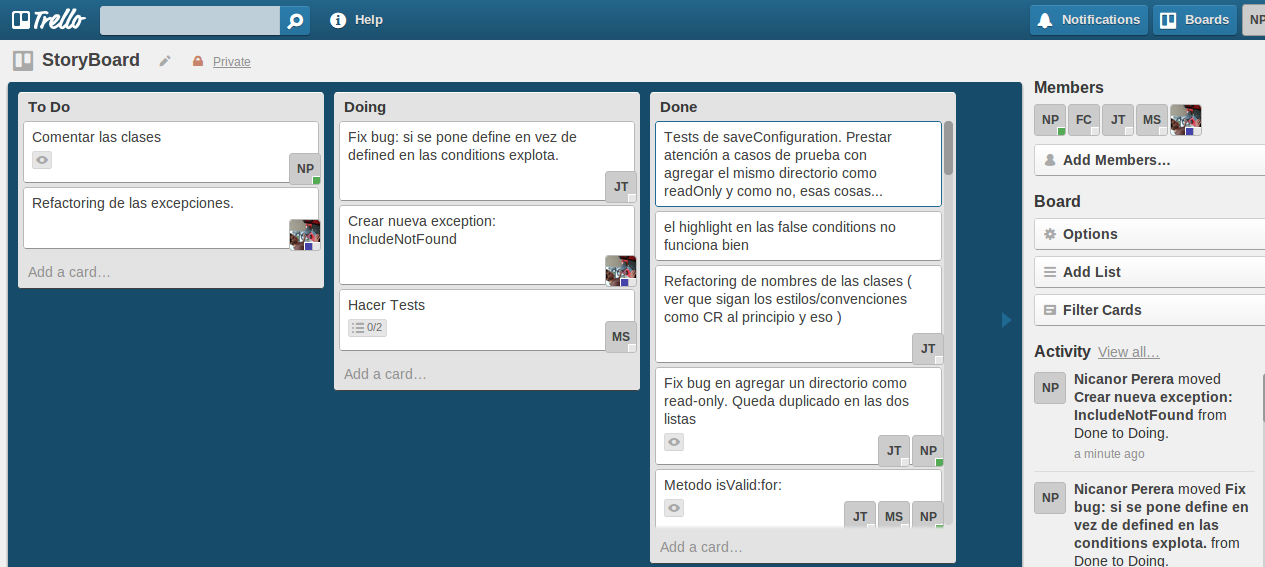
\includegraphics[scale=0.27]{images/trello.png}
    \caption{StoryBoard de Trello}
    \label{trello}
\end{figure}

Trello facilit\'o todas las tareas de organizaci\'on. Permit\'ia que cada uno pueda elegir su tarea sin superponerse con la de el otro, pod\'iamos ver lo que hac\'ia cada uno en tiempo real y colaborar para llevar a cabo las tareas de la forma mas eficientemente posible. 

Adem\'as realizamos tests autom\'aticos para validar que las funcionalidades m\'as importantes se ejecuten correctamente.

\section{Frameworks y herramientas utilizadas}
El proyecto est\'a implementado en Smalltalk, utilizando el entorno de desarrollo VisualWorks. Para realizar los tests utilizamos el framework SUnit.

Smalltalk es un lenguaje de programaci\'on orientado a objetos y de tipado din\'amico mientras que VisualWorks es una implementaci\'on multiplataforma de este lenguaje.

Sunit es un framework de tests de unidad para el lenguaje de programaci\'on Smalltalk. SUnit permite escribir tests y chequear resultados en Smalltalk.

\section{Diseño del proyecto}
Para realizar el proyecto tuvimos que extender y modificar algunas clases que componen la herramiena CRefactory. Las clases m\'as importantes que modificamos son las siguientes:
\begin{description}
\item[CRBrowser] Esta clase representa la ventana principal de la interfaz.
\item[CRConfigurationView] En esta clase esta imeplementada la interfaz para la gesti\'on de la configuraci\'on.
\item[CRErrorView] Esta clase se encarga se encarga de mostrar los mensajes de error cada vez que se produce una excepci\'on.
\item[CRConfigurationError] Esta es la clase base para el manejo de las excepciones. Aqu\'i se tienen datos como el archivo en el que se produjo el error o el n\'umero de l\'inea.
\item[CRPreparserError] Aqu\'i se manejan las excepciones producidas por errores en el preparser.
\item[CRParseError] Aqu\'i se manejan las excepciones producidas por errores en el parseo del c\'odigo fuente.
\item[CRIncludeNotFound] Aqu\'i se manejan las excepciones producidas por no haber encontrado una cabecera necesario.
\end{description}

\begin{figure}[h!]
  \centering
    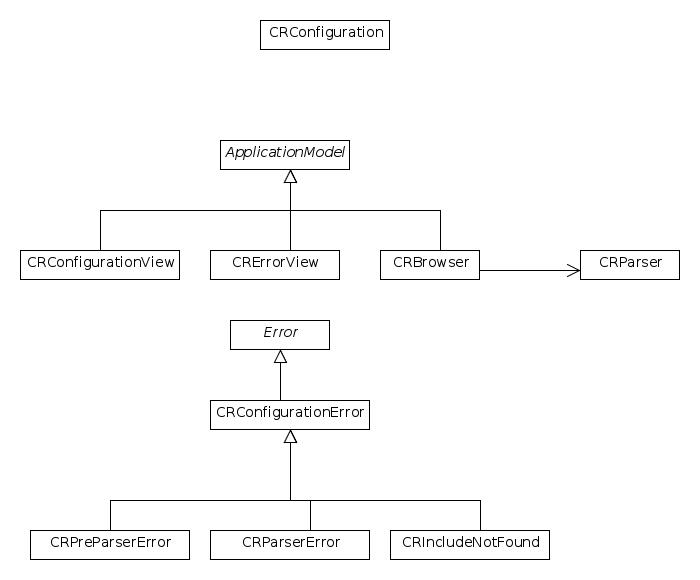
\includegraphics[scale=0.6]{images/diagrama_de_clases.jpg}
    \caption{Diagrama de clases}
    \label{diagrama_de_clases}
\end{figure}

\section{Problema uno: Carga de archivos}
\label{sec:problemOne}

El primer paso para trabajar con CRefactory es seleccionar los archivos de c\'odigo C al cual se le va a aplicar la refactorizaci\'on y las carpetas donde se encuentran los archivos de cabecera que incluyen dichos archivos (include directories).

Un archivo de cabecera es un archivo que el compilador incluye de forma autom\'atica al procesar alg\'un otro archivo fuente. Estos archivos contienen normalmente una declaraci\'on directa de clases, subrutinas, variables u otros identificadores.


\subsection{Contexto}
La carga de archivos en la interfaz original funcionaba de la siguiente manera:

\begin{figure}[h!]
  \centering
    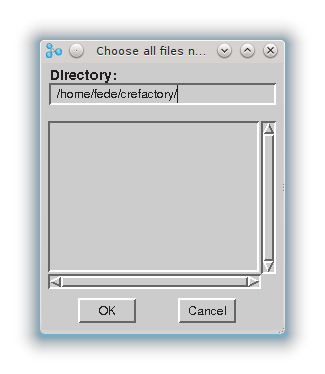
\includegraphics[scale=0.85]{images/codigo_original/carga.png}
    \caption{Carga de archivo original}
    \label{carga_original}
\end{figure}

Se deb\'ia escribir a mano el path absoluto hacia donde estaban los archivos. Esto era propenso a errores ya que se pod\'ian cometer errores de tipeo o incluso no recordar exactamente cual era dicho path.

Los path absolutos señalan la ubicaci\'on de un archivo o directorio desde el directorio ra\'iz del sistema de archivos.

Al cometer un error de tipeo o escribir el nombre de un archivo inexistente ocurr\'ia un error como el de la figura ~\ref{error} .

\begin{figure}[h!]
  \centering
    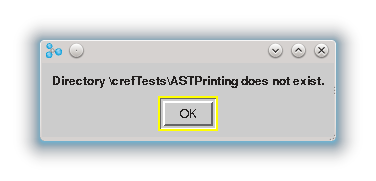
\includegraphics[scale=0.85]{images/codigo_original/error.png}
    \caption{Error}
    \label{error}
\end{figure}

\subsection{Soluci\'on planteada}
El problema se solucion\'o agregando una ventana de exploraci\'on de archivos. Este permiti\'o explorar el filesystem y seleccionar el archivo deseado. Ahora se podr\'ia seleccionar m\'as de uno al mismo tiempo.
Las ventajas de esta aproximaci\'on son que es menos propensa a errores y el usuario no necesita recordar el path absoluto.

En la Figura ~\ref{carga_archivo} mostramos un pantallazo de la visualizaci\'on de la nueva ventana de exploraci\'on de archivos.

\begin{figure}[h!]
  \centering
    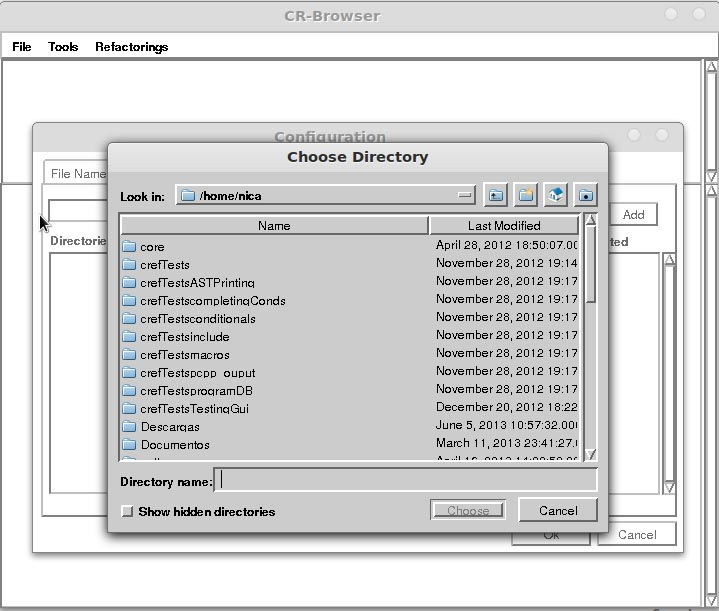
\includegraphics[scale=0.50]{images/codigo_modificado/seleccionar_directorio.jpg}
     \caption{Carga de archivo}
     \label{carga_archivo}
\end{figure}

\section{Problema dos: Configuraci\'on}

Un archivo fuente de c\'odigo C no s\'olo contiene sintaxis del lenguaje, sino que puede, y suele, contener directivas al preprocesador, tales directivas brindan la posibilidad de realizar inclusi\'on de archivos, definici\'on de macros o compilaci\'on condicional.

La inclusi\'on de archivos permite tener un programa alojado en varios archivos distintos por lo que una refactorizaci\'on podr\'ia tener un alcance mayor al archivo que se est\'a visualizando en ese momento.

Una macro es una forma de sustituir caracteres por otros, las macros constan de un nombre y un cuerpo, durante el preprocesado cada ocurrencia del primero ser\'a reemplazado por el segundo. El cuerpo de la macro puede referir directamente a elementos globales del programa o hacerlo indirectamente, a trav\'es de la concatenaci\'on de s\'imbolos, lo que puede f\'acilmente violar la correctitud de una refactorizaci\'on.

La compilaci\'on condicional proporciona una forma de incluir c\'odigo selectivamente dependiendo del valor de determinadas condiciones en tiempo de compilaci\'on, lo que puede derivar en m\'ultiples ramas que son mutuamente exclusivas, si durante una refactorizaci\'on s\'olo se considera una de ellas las otras pueden volverse obsoletas o erroneas y si por el contrario todas las ramas son consideradas cada elemento puede tener m\'ultiples definiciones, como una variable con m\'ultiples tipos.

Dado que la herramienta CRefactory puede realizar operaciones de refactorizaci\'on sobre c\'odigo sin preprocesar es necesario otorgarle cierta informaci\'on extra que le permita a la herramienta resolver situaciones dificiles de manejar a la hora de refactorizar, \'esta informaci\'on es llamada configuraci\'on. En concreto la configuraci\'on necesaria es:

\begin{itemize}
\item Directorios d\'onde se encuetran los archivos inclu\'idos por el archivo cargado.
\item Cuerpos de macros.
\item Condiciones falsas para determinar que ramas de c\'odigo deben ser tenidas en cuenta y cuales no a la hora de refactorizar.
\end{itemize}

\subsection{Contexto}
La interfaz de CRefactory permit\'ia, como se dijo en la secci\'on ~\ref{sec:problemOne}, ingresar los directorios d\'onde se alojan los archivos inclu\'idos por el archivo a editar, pero no brindaba la posibilidad de definir cuerpos de macros ni de espec\'ificar condiciones falsas por lo cual era necesario extender la GUI para proveer esa funcionalidad.

\subsection{Soluci\'on planteada}
Se decidi\'o implementar una nueva ventana que servir\'ia de interfaz para ingresar la informaci\'on de configuraci\'on. Dado que ya exist\'ian dos ventanas de dialogo para realizar parte de la configuraci\'on (la selecci\'on de los archivos fuente a editar y la especificaci\'on de la ubicaci\'on de los archivos includ\'idos por dichos fuentes) se opt\'o por no sobrecargar la vista agregando un tercer di\'alogo, o quizas m\'as teniendo en cuenta que se necesitaba brindar la posibilidad de definir tanto macros como condiciones falsas, sino unificar todos \'estos aspectos relacionados en una sola vista. Por \'ultimo nos inclinamos a utilizar una vista  con solapas dado que una sola ventana con tanta informaci\'on podr\'ia resultar confusa y se dificultar\'ia encontrar r\'apidamente d\'onde ingresar la informaci\'on de configuraci\'on deseada, por otro lado mucha de esa informaci\'on s\'olo ser\'a necesaria en algunos casos, por ejemplo muchas veces se podr\'a editar un archivo donde no fuera necesario definir macros, por lo que la vista en solapas se ajusta a la necesidad de s\'olo mostrar lo necesario y no m\'as que eso, quien no necesite definir macros puede simplemente obviar esa solapa.

El resultado final fue entonces el mostrado en la figura~\ref{configuracion}

\begin{figure}[h!]
  \centering
    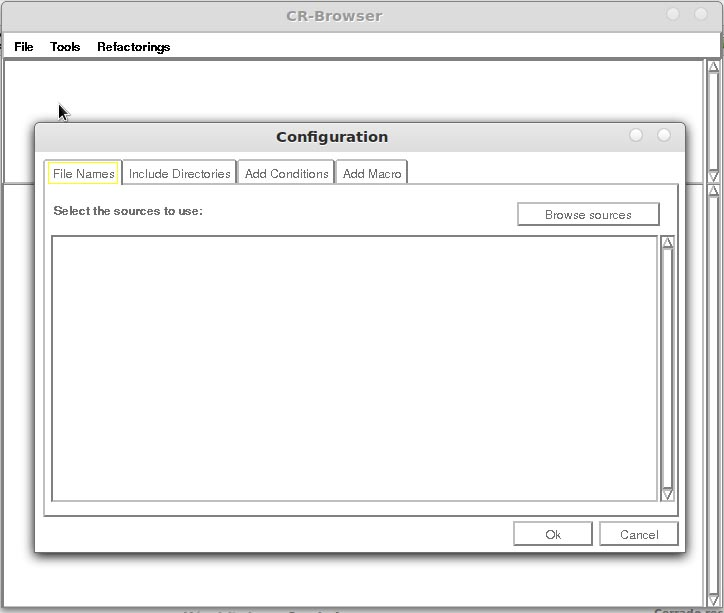
\includegraphics[scale=0.45]{images/codigo_modificado/configuracion.jpg}
     \caption{Interfaz de configuraci\'on}
     \label{configuracion}
\end{figure}

\section{Problema tres: Manejo de excepciones}

El manejo de excepciones es una t\'ecnica de programaci\'on que permite controlar los errores ocasionados durante la ejecucici\'on del programa.
A continuaci\'on se detallan los problemas que presentaban la ausencia del manejo de estas en la interface de CRefactory y como fueron solucionados estos problemas.

\subsection{Contexto}
Ante un error de parseo la aplicaci\'on dejaba de funcionar. No hab\'ia ning\'un tipo de manejo de excepciones. No encontrar un archivo de cabecera en los directorios incluidos significaba que el programa se cerrara abruptamente, sin ning\'un tipo de retroalimentaci\'on para que el usuario pueda rastrear el error. Se hizo evidente la necesidad de que el usuario pudiera rastrear el error y corregirlo sin que falle la herramienta.

\begin{figure}[h!]
  \centering
    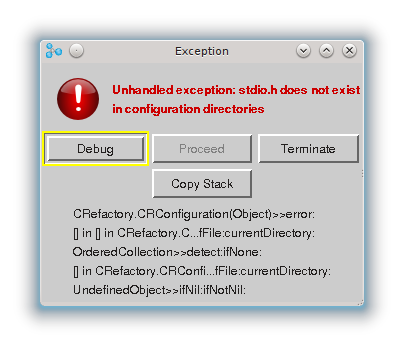
\includegraphics[scale=0.85]{images/codigo_original/error_header_no_agregado.png}
     \caption{Error por header no incluido}
     \label{header_no_incluido}
\end{figure}

\subsection{Soluci\'on planteada}
Lo que se hizo en un principio fue implementar los manejadores para las excepciones. Por lo que cuando se produc\'ia una excepci\'on se mostraba una ventana con una descripci\'on del error ayudando al usuario para que puediera corregirlo. Por ejemplo, cuando no se inclu\'ia el directorio donde buscar una cabecera se mostraba una ventana que advert\'ia al usuario del error y le daba la posibilidad de corregirlo agregando el directorio necesario en la ventana de configuraci\'on.

En la Figura ~\ref{header_no_encontrado} se ve como se mostraba el error luego de implementar el manejo de excepciones.

\begin{figure}[h!]
  \centering
    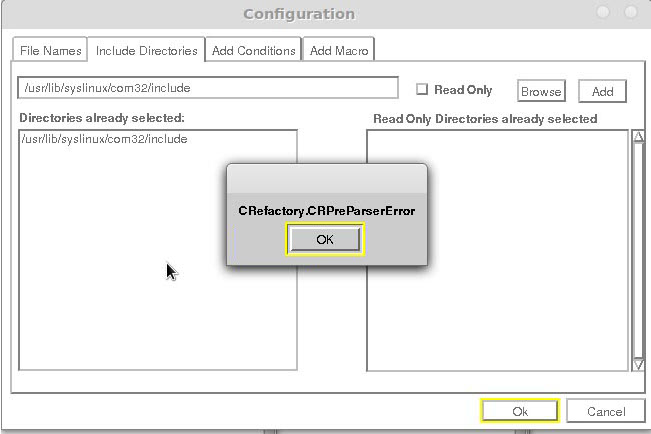
\includegraphics[scale=0.50]{images/codigo_modificado/error_header_no_encontrado_sin_view_error.jpg}
     \caption{Error por header no encontrado}
     \label{header_no_encontrado}
\end{figure}

\section{Problema cuatro: Ventana de error}

Al ocurrir una exepci\'on no hab\'ia manera de que el usuario puediera tratarla. Se vi\'o la necesidad de visualizar el problema gr\'aficamente a trav\'es de una ventana de error

Una ventana es un \'area visual que contiene alg\'un tipo de interfaz de usuario, mostrando la salida y permitiendo la entrada de datos para los procesos en ejecuci\'on. Las ventanas pueden ser manipuladas con un puntero.

A continuaci\'on se explica como se trataba antes la excepci\'on, que problemas tra\'ia esto y como fueron solucionados.

\subsection{Contexto}
El problema de la soluci\'on planteada en el punto anterior es que no mostraba en que parte del c\'odigo fuente se produjo el error. Por lo tanto el usuario no siempre pod\'ia recuperarse totalmente.

\subsection{Soluci\'on planteada}
\'Esto llev\'o a reemplazar la ventana de notificaci\'on de error por una que diera la posibilidad de visualizar el c\'odigo fuente informando el error que se produjo. En la Figura ~\ref{ventana_de_error} se muestra una imagen de la ventana mostrando el error.

\begin{figure}[h!]
  \centering
    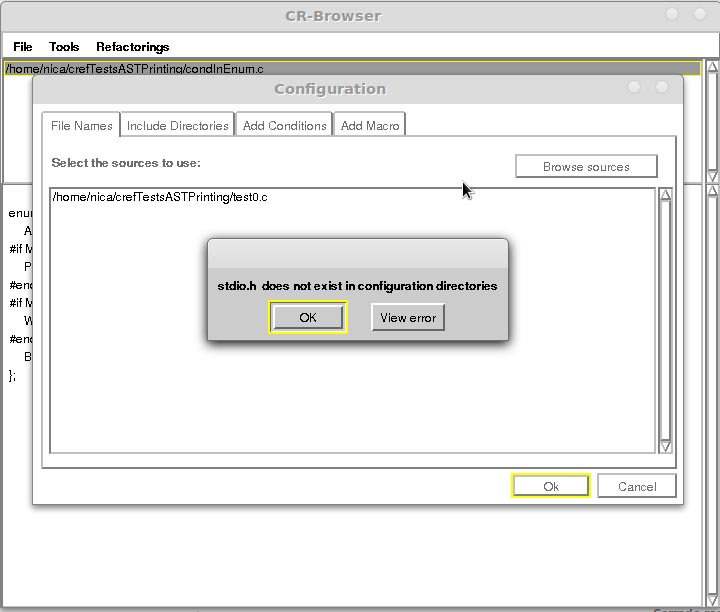
\includegraphics[scale=0.50]{images/codigo_modificado/error_header_no_encontrado.jpg}
     \caption{Ventana de error}
     \label{ventana_de_error}
\end{figure}

\section{Problema cinco: Highlight del error}

Cuando ocurre un error es \'util conocer que linea o lineas de c\'odigo son las que lo provocaron. Para poder identificar una porci\'on de c\'odigo, estuvimos de acuerdo en que ser\'ia muy \'util contar con alg\'un tipo de resaltado de texto. A continuaci\'on se explica c\'omo se mostraba el c\'odigo antes, que problemas tra\'ia \'esto y c\'omo fueron solucionados.

\subsection{Contexto}
Anteriormente, luego de un error se mostraba el c\'odigo pero no era claro que l\'ineas lo hab\'ian producido. Esto era un problema ya que la idea del manejo de excepciones no es solo identificar el error sino encontrar la manera de solucionarlo. Y muchas veces para solucionar un problema es necesario saber exactamente en que porci\'on del c\'odigo se origin\'o.

\subsection{Soluci\'on planteada}
El problema se solucion\'o implementando en la interfaz el resaltado de las l\'ineas donde se produjo el error. Gracias a \'esto el programador puede solucionar los errores con mucha mayor facilidad.

En la Figura ~\ref{resaltado} se visualiza el resaltado de un error.
\begin{figure}[h!]
  \centering
    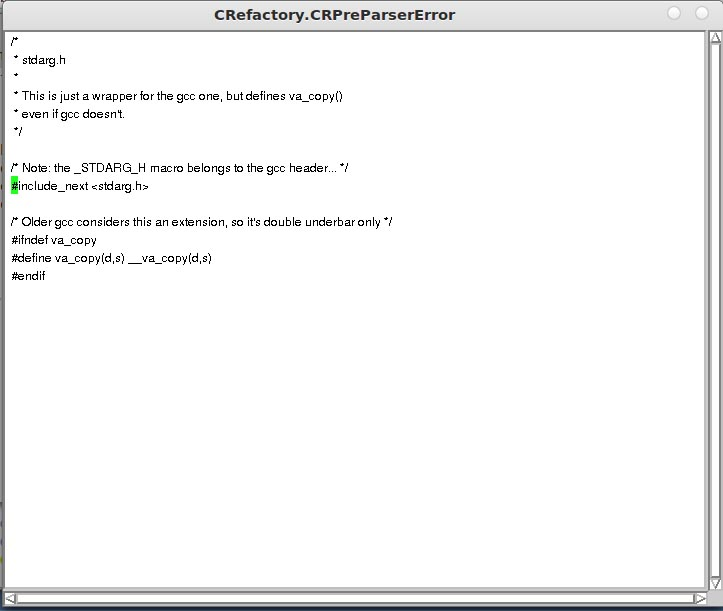
\includegraphics[scale=0.50]{images/codigo_modificado/highlight_preparser.jpg}
     \caption{Resaltado del error}
     \label{resaltado}
\end{figure}


\section{Instrucciones de instalaci\'on y uso}

\begin{enumerate}
\item Instalar VW7.8nc
\item Abrir la imagen, guardarla con nuevo nombre y setear el VisualWorks home directory

\item Desde el Parcel Manager cargar:
  \begin{itemize}
  \item All Advanced Tools
  \item RBSUnitExtensions
  \end{itemize}
  
\item Conectarse al repositorio Store de la c\'atedra: catedras.lifia.info.unlp.edu.ar:5432\_tpoo y buscar entre los “Published Items” el Bundle CRefactory. Instalar la ultima version (1.4) y luego instalar el bundle CRefactoryGUI.

\item Lo siguiente es probar que los tests de CRefactory pasen correctamente. Estos tests crean archivos .c de prueba en un directorio que deben especificar. Para esto browsear el c\'odigo de: “CRefactory-Testing-Root”, clase “CREFTestCase”, m\'etodo de clase “codeDirectory” y editarlo haciendo referencia a un directorio ya creado en la m\'aquina.
  
\item Seleccionar el package {\it CRefactory-Testing} y correr todos los tests. Deber\'ian pasar los 173 tests.

\item Para correr la aplicaci\'on debemos ejecutar en el \'area de trabajo  {\it CRBrowser open}. 
\end{enumerate}

\section{Minutas}
Durante el desarrollo del proyecto tuvimos varias reuniones con la Profesora, con la finalidad de conocer cu\'ales eran los requerimientos y mostrar el avance del proyecto. Cada vez que ten\'iamos una reuni\'on deb\'iamos tomar apuntes de lo que hab\'iamos hablado.

A continuaci\'on presentamos dichos apuntes o minutas:

\subsection{Reuni\'on del Lunes 10/09}
La Profesora nos di\'o una breve introducci\'on al proyecto y un vistazo general de c\'omo est\'a organizado. Nos explic\'o c\'omo estaba funcionando hasta ese momento. Aprendimos c\'omo cargar el proyecto dentro de visualworks y a realizar todas las configuraciones necesarias para el correcto funcionamiento de la aplicaci\'on.

Nos explic\'o c\'omo conectarnos al repositorio de la c\'atedra y c\'omo utilizar la herramienta de control de versiones.
Acordamos que nos enviar\'ia por correo electr\'onico los nombres de usuarios y contraseñas de cada integrante del grupo para acceder al repositorio.

Luego de \'esta introducci\'on al proyecto hablamos las funcionalidades que tendr\'iamos que implementar a lo largo de la cursada. Las m\'as importantes:

\begin{itemize}
  \item Mejorar el di\'alogo de carga de un archivo. Que sea por ejemplo como el de carga de parcels, haciendolo m\'as accesible al usuario.
  \item Poder especificar donde estan los directorios con los headers.
  \item Tener en cuenta las configuraciones que no se pueden parsear.
  \item Manejar las excepciones para que cuando hay una configuraci\'on inv\'alida muestre en el c\'odigo donde esta lo inv\'alido. 
\end{itemize}

Adem\'as se coment\'o que ser\'ia interesante como trabajo a futuro, posibilitar la creaci\'on autom\'atica de grafos de la inclusi\'on de archivos.

\subsection{Reuni\'on del Lunes 17/09}
En \'esta reuni\'on la Profesora nos enseñ\'o c\'omo funcionaba el di\'alogo de carga de archivos. Anteriormente era necesario escribir el nombre de los archivos a incluir, lo cual hac\'ia tedioso el trabajo y ocurr\'ia que ante un error de tipeo no se encontrar\'ia el archivo y el programa cerrar\'ia abruptamente. 

Planteamos modificar el di\'alogo de carga de archivo para que permita explorar el file system. De esta manera ser\'ia m\'as f\'acil de utilizar y se solucionar\'ian los problemas.

\subsection{Reuni\'on del Jueves 18/10}
Para este momento ya hab\'iamos implementado la carga de archivos y directorios por medio de un File Browser, pero todav\'ia no era el ideal.

En esta reuni\'on se habl\'o con la Profesora sobre la necesidad de marcar a algunos directorios como directorios de s\'olo lectura (Read Only).

Tambi\'en hablamos sobre la implementaci\'on de manejo de excepciones. En particular ocurr\'ia frecuentemente una excepci\'on al no incluir los directorios necesarios. Acordamos implementar el manejo de dicha excepci\'on.


Adem\'as comentamos los siguientes puntos:
\begin{itemize}
 \item Mejorar la secci\'on include Directory, para que se puedan agregar directamente.
 \item Bajar un ejemplo opensource en C para probar el funcionamiento.
 \item Prestar atenci\'on a preprocess y a FullNameOfFile.
\end{itemize}

\subsection{Reuni\'on del Lunes 29/10}
En esta reuni\'on comenzamos a hablar sobre el tratamiento de excepciones en CRefactory. La Profesora nos aconsej\'o que leamos la documentaci\'on del manejo de excepciones en Visual Works y que miraramos ejemplos en su c\'odigo fuente para elegir la estrategia a utilizar.

Cuando se produc\'ia un error, CRefactory no indicaba cu\'al era el archivo que lo hab\'ia producido. Nos propusimos como objetivo que se pueda mostrar dicho archivo, y resaltar la l\'inea de c\'odigo en la cu\'al se produjo el error.

\subsection{Reuni\'on del Lunes 12/11}
Durante la implementaci\'on de las diferentes funcionalidades, no tuvimos en cuenta el correcto funcionamiento de la aplicaci\'on, y descubrimos que algunas cosas hab\'ian dejado de funcionar. La Profesora nos sugiri\'o que nos asegur\'aramos de que pasen los tests de CRefactory. Nos propusimos realizar tests de todas las funcionalidades importantes que implementaramos.

Los errores de parseo en presencia de condiciones falsas sol\'ia ser un problema, ya que muchas veces se dificultaba encontrar el lugar donde ocurr\'ia el error. La Profesora plante\'o resolverlo y nos recomend\'o comenzar probando con el archivo test19.c.

\subsection{Reuni\'on del Jueves 29/11}
En esta reuni\'on volvimos a hablar acerca de los problemas vinculados con las condiciones falsas. Se nos pidi\'o tener la posibilidad de cachear la excepci\'on que ocurr\'ia al agregar una condici\'on falsa y se nos sugiri\'o investigar la implementaci\'on de la clase Preprocessor.

\section{Conclusiones}
En esta secci\'on explicaremos los logros alcanzados durante el proyecto, los valores que obtuvimos y algunas sugerencias para un futuro trabajo de CRefacory.

\subsection{Logros alcanzados}
La nueva interfaz es pr\'actica para cargar archivos, directorios, macros y condiciones falsas. Ahora se pueden cargar archivos de forma segura. En lugar de escribir el nombre del archivo o directorio se lo puede seleccionar entre los ya existentes. 

Ahora es posible acceder a funcionalidades que antes no se pod\'ian, como por ejemplo la posibilidad de agregar condiciones falsas a la configuraci\'on para que no sean parseadas.

Cambiamos el diseño de la interfaz de manera que sea, a nuestro criterio, mucho m\'as amigable con el usuario.

Al dispararse una excepci\'on de parseo, la nueva interfaz ahora permite detectar la l\'inea de c\'odigo en la cual ocurri\'o.

\subsection{Valores obtenidos}
Trabajamos utilizando una metodolog\'ia \'agil de tipo Scrum. \'Esto nos permiti\'o tener una buena organizaci\'on. Ayud\'o al trabajo en equipo, optimiz\'o la eficiencia en la resoluci\'on de las tareas.

Comprendimos la importancia de realizar tests automatizados durante la programaci\'on. Si bien nos demor\'o implementar el c\'odigo de los tests, creemos que a la larga salimos beneficiados con respecto a la distribuci\'on del tiempo. Adem\'as saber que el programa segu\'ia funcionando nos daba mucha m\'as seguridad al programar.

\subsection{Trabajo futuro}
En orden de conseguir que CRefactory sea una herramienta profesional que pueda competir con otros productos similares creemos que se debe soportar las siguientes caracter\'isticas:

\subsubsection{Coloreado de Sintaxis}
El coloreado de sintaxis es una caracter\'istica muy com\'un en los editores de texto modernos, consiste en mostrar el c\'odigo fuente en diferentes colores con el objetivo de mejorar la legibilidad del c\'odigo para el programador.

\subsubsection{Localizaci\'on autom\'atica de c\'odigo refactorizable}
Actualmente, para refactorizar c\'odigo, el programador debe identificar el problema observando el c\'odigo. Creemos que ser\'ia buena idea implementar un algor\'itmo que sirva para localizar c\'odigo potencialmente refactorizable de manera autom\'atica.

\subsubsection{Integraci\'on con frameworks de testing}
Al refactorizar c\'odigo, debemos comprobar que el c\'odigo siga funcionando correctamente. Ser\'ia deseable que CRefactoring tenga integrados frameworks de testing para realizar el testeo del c\'odigo de forma autom\'atica.

\subsubsection{Personalizaci\'on del entorno}
Ser\'ia bueno otorgar a la interface cierta flexibilidad para poder adaptarse a las necesidades de cada usuario.


\subsubsection{Formateo autom\'atico de c\'odigo}
El formateo de c\'odigo es una herramienta que permite modificar el c\'odigo para que \'este se presente siguiendo convenciones de identaci\'on, espaciado y posicionamiento. \'Esto ayuda a que el c\'odigo sea m\'as f\'acil de leer, entender y mantener para el desarrollador.

Creemos que ser\'ia ideal que CRefactory cuente con una herramienta de formateo autom\'atico.


\subsubsection{Tabla de s\'imbolos}
Una tabla de s\'imbolos es una estructura de datos donde cada s\'imbolo en el c\'odigo fuente de un programa est\'a asociado con informaci\'on, como por ejemplo la ubicaci\'on, el tipo de datos y el \'ambito de cada variable.

Ser\'ia bueno poder ver la tabla de s\'imbolos.

\subsubsection{Grafo de dependencias}
Puede ser \'util visualizar las dependencias del c\'odigo fuente. Ser\'ia interesante contar con una herramienta que realize grafos de inclusi\'on de archivos de forma autom\'atica.

\end{document}